\chapter{\acs{rfid} Smart Shelves}

\ac{rfid} enabled smart shelves, or intelligent shelves, are shelves, racks or cabinets that are equipped with \ac{rfid} capabilities.
Tagged objects placed on these shelves can be inventoried and monitored in real-time, to solve common problems related with inventory management.

Smart shelves solve a multitude of problems across multiple industries. A few advantages offered by smart shelves are listed bellow~\cite{lahiriRFIDSourcebook2005, WhatYouNeed, FutureRetailShopping, SmartShelvesKey2019}:

\begin{itemize}
    \item Get timely accurate replenishment of products, avoiding stock-outs and better management of inventory. It can ensure availability of products and automated control of expiration dates, useful in multiple industries to keep accurate stock information and control of products. In markets of volatile products (e.g.\ low quantity batches, perishable goods with short shelf life, products with high volatile prices), \ac{rfid} services can ensure timely delivers and automation of orders.
    \item Optimise in-store sales and management by reducing time and errors from manual labour counts, identify misplaced and lost or stolen items. Bridges online and physical stores inventories, maintaining accurate visibility of product availability. \ac{rfid} also helps customers find and engage with the products they want.
    \item In industries working with valuable tools and materials (e.g.\ hospitals, research centers), it can help control who removes or checks out valuable items, and locate them in a timely manner.
    \item Enable retailers to better understand product sale potential, by analysing data generated from smart shelves displaying sale items.
    \item Create visibility and automate \ac{scm}. Enterprise back-end systems (e.g.\ machine learning services) can infer and automate optimal product distribution, predict market changes and necessities, that otherwise had to be anticipate by management teams.
\end{itemize}


\section{Commercial Solutions}

There are multiple commercial \ac{rfid} smart shelves available on the market.
The most prominent sector has been the health industry, with smart \ac{rfid}-enabled cabinets~\cite{RFIDSmartCabinets, RFIDTechnologyCabinet, DyaneSmartCabinetSmart,RFIDEnabledCabinetry}, where in conjunction with technologies like the \emph{EPCGlobal Pedigree} standard~\cite{PedigreeStandardV1}, maintains accurate inventory and ensures only authentic pharmaceutical products are distributed through the supply chain.
In the following subsections, I will presented generic smart shelves currently commercialized which use \ac{rfid} in their solution.

\subsection{Keon: AdvanShelf™}

Keonn, a leader in \ac{uhf} \ac{rfid} systems for retail stores and intelligent spaces, commercializes the \emph{AdvanShelf™}.
The \emph{AdvanShelf™} is a \ac{uhf} smart shelve system design for real-time location of items~\cite{AdvanShelfRFIDSmart}.
The system was designed to be invisible, incorporated into metallic, plastic and wood-made shelves.
It includes an \ac{rf} multiplexer, which can connect up to $1024$ antennas to one reader, location software with a resolution of $\pm40$~cm and Keonn Java drivers for system integration.

They also commercializes \ac{rfid}-enabled lockers, shown on figure~\ref{fig:keonnlocker}, based on the \emph{AdvanShelf™} \ac{rfid} solution of readers, antennas and multiplexers.

\begin{figure}[!ht]
    \centering
    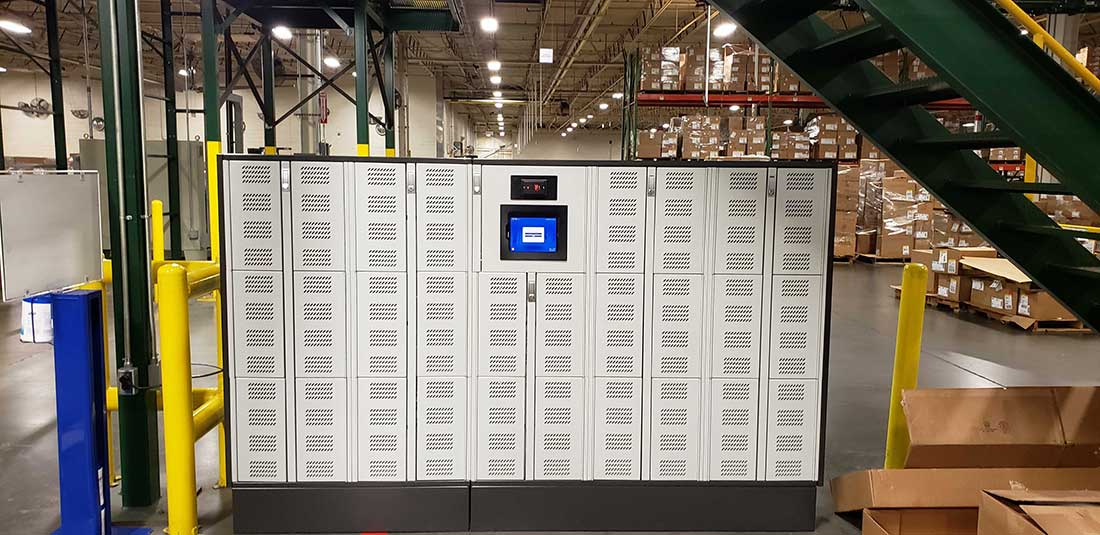
\includegraphics[width=1\textwidth]{./figs/02-state-of-the-art/keonn_lockers.jpg}
    \caption[\ac{rfid}-based electronic lockers from Keonn]{\ac{rfid}-based electronic lockers from Keonn based on the \emph{AdvanShelf™} solution~\cite{RFIDenabledLockersProvide}} 
    \label{fig:keonnlocker}
\end{figure}

\subsection{CribMaster: AccuCab and AccuDrawer}

CribMaster, a company focused on intelligent inventory management, mainly for industrial hardware, commercializes two inventory systems: \emph{AccuCab} and \emph{AccuDrawer}.
The \emph{AccuCab}, shown in figure~\ref{fig:cribmasteraccucab}, is their solution for tool access and storage. It has pull-out shelving for easy access, and is ideal for storing heavy items like power and hand tools.
The \emph{AccuDrawer}, shown in figure~\ref{fig:cribmasteraccydrawer}, is the same product in a drawer configuration.
They use passive \ac{rfid} tags, and no further specifications are given.

\begin{figure}[!ht]
    \centering
    \begin{subfigure}{.45\textwidth}
        \centering
        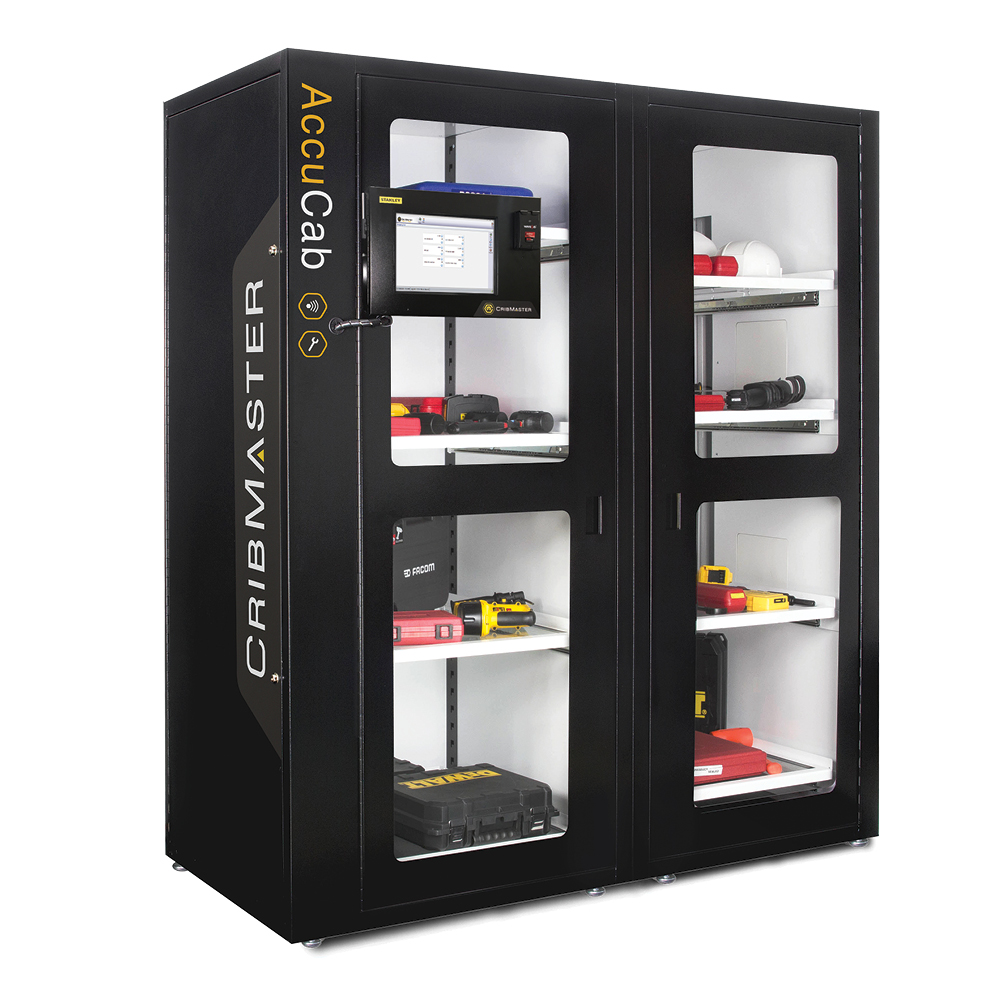
\includegraphics[width=\linewidth]{./figs/02-state-of-the-art/cribmaster2.jpg}
        \caption[CribMaster AccuCab inventory system cabinet solution]{CribMaster AccuCab inventory system cabinet solution~\cite{AccuCabCribmasterCom}} 
        \label{fig:cribmasteraccucab}
    \end{subfigure}
    \begin{subfigure}{.45\textwidth}
        \centering
        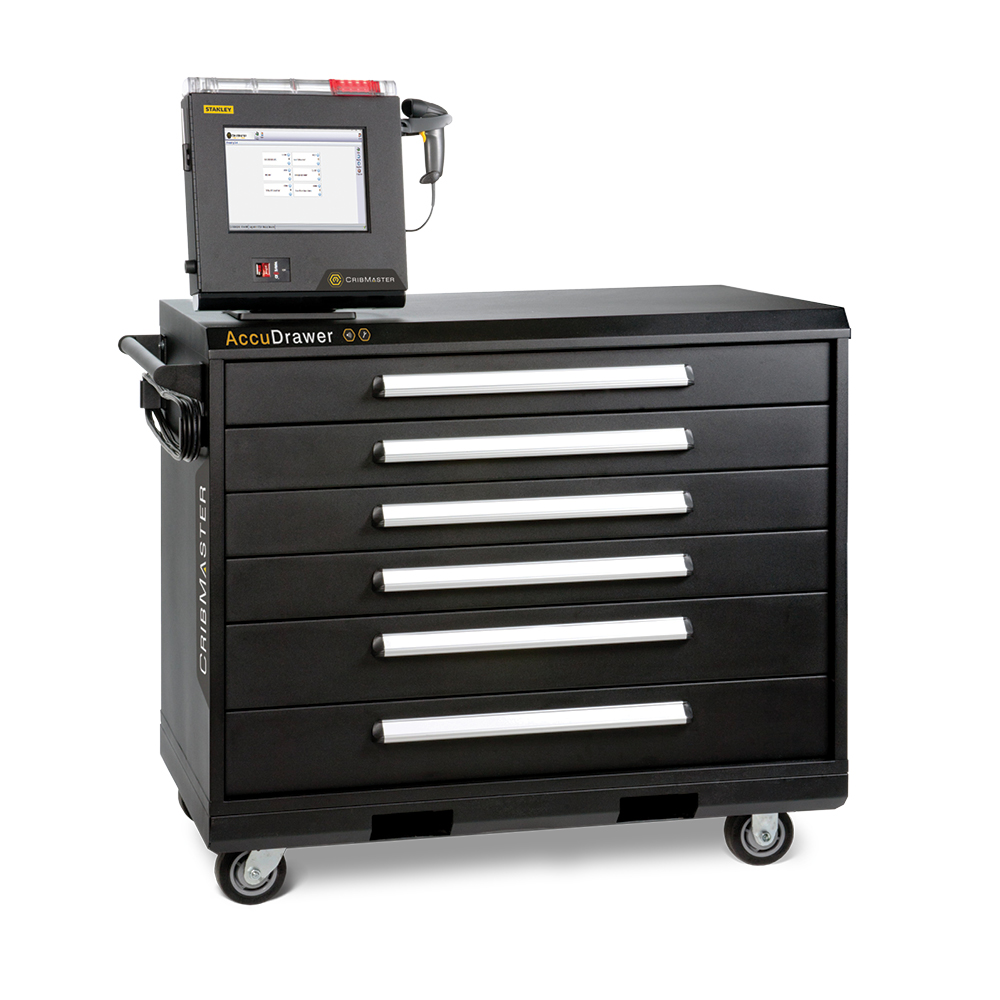
\includegraphics[width=\linewidth]{./figs/02-state-of-the-art/cribmaster1.jpg}
        \caption[CribMaster AccuDrawer smart storage control]{CribMaster AccuDrawer smart storage control~\cite{AccuDrawerCribmasterCom}} 
        \label{fig:cribmasteraccydrawer}
    \end{subfigure}
    \caption[CribMaster \ac{rfid} inventory management systems]{CribMaster \ac{rfid} inventory management systems} 
    \label{fig:cribmaster}
\end{figure}

\subsection{Fabmatics: \ac{rfid} Rack}

Fabmatics is a company specialized in material flows and handling processes in industries with high cleanliness requirements (e.g.\ semiconductor industry, pharmaceutical industry, photovoltaics and large-scale laboratories), where it integrates their products in the client's production environment~\cite{RFIDRackFabmatics}.
They offer a retrofitted \ac{rfid} storage systems for silicon wafers, shown in figure~\ref{fig:fabmaticsrfidrack}.
No further technological specifications referring to \ac{rfid} are presented.

\begin{figure}[!ht]
    \centering
    \begin{subfigure}{.45\textwidth}
        \centering
        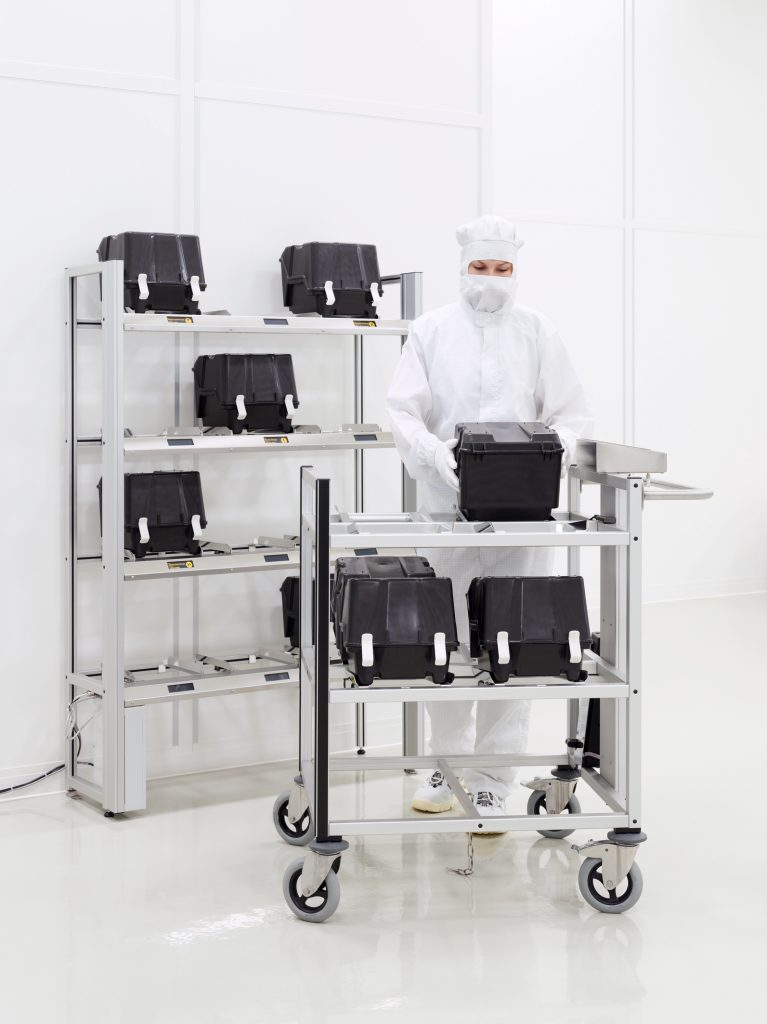
\includegraphics[width=\linewidth]{./figs/02-state-of-the-art/fabmaticsrfidrack2.jpg}
    \end{subfigure}
    \begin{subfigure}{.45\textwidth}
        \centering
        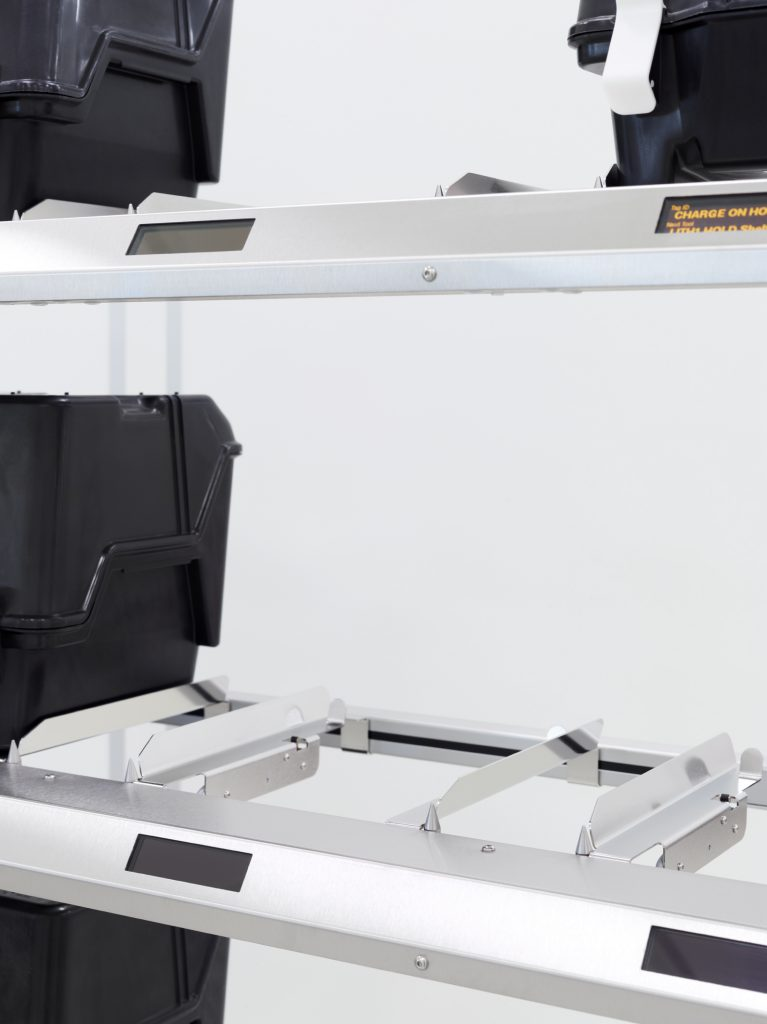
\includegraphics[width=\linewidth]{./figs/02-state-of-the-art/fabmaticsrfidrack3.jpg}
    \end{subfigure}
    \caption[Fabmatics \ac{rfid} Rack design for wafer storage]{Fabmatics \ac{rfid} Rack design for wafer storage~\cite{RFIDRackFabmatics}} 
    \label{fig:fabmaticsrfidrack}
\end{figure}

Many smart shelves in the market do not depend on \ac{rfid} to do inventory, but on other technologies like image processing, \ac{iot} and machine learning to do so~\cite{TechnologyWiseShelf, RetailSolutionsAWM}.

\section{Academic solutions}

Smart shelves have been approached by a few students and researchers in their work over the years. Overall, the research had targeted antenna design and item location. Nothing was found on smart shelve \emph{EPCGlobal Framework} integration.

The prominent applications of smart shelves, by academic resources over the years, has been focused in the health industry, with smart cabinets~\cite{shiehUsingRFIDTechnology2008, dalessandroRFIDBasedSmartShelving2012, medeirosUHFRFIDCabinet2011, gomesIntelligentMedicineCabinet2013} and \ac{rfid}-based smart blood stock system~\cite{zaricRFIDbasedSmartBlood2015}, and in \ac{rfid} library managements systems~\cite{markakisRFIDenabledLibraryManagement2013, markakisSafeEfficientDesign2014, ahmadtarmizibinabdullahLibraryShelfManagement2011, nishiyamaSmartShelfEfficient2012}.

For more generic implementations, Andrea D’Alessandro, in his PhD thesis, has studied and developed \ac{uhf} \ac{rfid}-based smart shelving storage systems with location capabilities~\cite{dalessandroRFIDBasedSmartShelving2012}.
He studied location techniques for \ac{uhf} \ac{rfid} smart shelves, employing ``off the shelf'' hardware components in different arrangements.

Other researches employed similar techniques to identify and locate items on shelves, mainly focusing on antenna design applications and item location techniques~\cite{choiPassiveUHFRFIDBased2012, nikitinTheoryMeasurementBackscattering2007, medeirosUHFRFIDReader, yuanUHFRFIDShelf2012a}. 
In particular, over the last years, a huge amount of study has been put in development and research of antennas for \emph{near-field} \ac{uhf} \ac{rfid}, intended to be used in smart shelves and similar purposes~\cite{yuanUHFRFIDShelf2012a, liCIRCULARLYPOLARIZEDCOMPACT2013, casoModularAntennaUHF2014, ankangrenNovelDesignUHF2010, michelScalableModularAntenna2015, michelOverviewModularAntennas2016, michelDesignPerformanceAnalysis2012, parthibanLowcostScalableUHF2016, andrenkoNovelDesignUHF2013, choPlanarNearFieldRFID2011, tolinPolarizationReconfigurablePatch2019, parthibanScalableNearfieldFed2019, chenDesignSimulationUHF2018, choiUshapedSlotarrayAntenna2011, liUHFRFIDShelf2017, yuanUHFRFIDShelf2012, manziUseTransmissionLines2012, catarinucciImprovingItemlevelTracing2010, guDesignNearFieldRFID2019}.
A lot of time was invested in research of this topic throughout the beginning of this dissertation, but abandoned in favor of implementing a prototype which integrates the \emph{EPCGlobal Architecture Framework} technologies.

There have been a few out of the box implementations using $3D$ localization of \ac{uhf} \ac{rfid}-tagged products by ground robots and drones with commercial off-the-shelf \ac{rfid} hardware~\cite{tzitzisRealtime3DLocalization2020}.

Research was also put on developing cheaper and better open \ac{uhf} hardware based on commercial \ac{ic} chips~\cite{tangDesignUHFRFID2010a, leiDesignHandheldUHF2011, wangHardwareDesignImplementation2015} and \acp{fpga}~\cite{mirandaSistemasRFIDUHF2015}.

In the next chapter I will address dissertation requirements, present development options and their peculiarities in respect to performance, cost and development time.

\cleardoublepage